\section{Domain Formalization}
\label{sec:Domain}

The foundation of any systematic approach for domain-specific-DSE is the formalization of a domain and its features (metrics) to quantitatively reason about the domain. This section defines the domain scope and its features (metrics). They capture the behavioral and structural features of a domain showing what functions are commonly used and how they are composed. Defining these features and metrics lays the foundation for automatic domain analysis and exploration.

\subsection{Domain Definition}
\label{sub:dmDefine}
Domain is a set of applications, which share common functions and common patterns\cite{kang1990feature}. To allow reasoning about the domain\footnote{Defining the scope of a domain, i.e. assessing domain membership, is an additional research topic.}, we formally define it as a set of graphs.
%Current definitions of domain include a set of applications which share a set of common capabilities and data \cite{kang1990feature}, a class of applications, with a component library, which contains reusable chunks of domain expertise \cite{tracz1995dssa}. Following this definition, we define a domain as a set of applications, which share common functions and common patterns. To allow reasoning about the domain\footnote{Defining the scope of a domain, i.e. assessing domain membership, is an additional research topic.}, we formally define it as a set of graphs.
%\vspace{-5pt}
\begin{equation}
\begin{split}
\label{eq:domain}
	&G = \{g_{0}, g_{1}, ..., g_{N}\}, \quad g_{i} = (A, E)\\
	&A = \{a_{0}, a_{1}, ..., a_{n}\}, \quad E = \{e_{0}, e_{1}, ..., e_{m}\}\\
	&a_{i} (t, d_{P}), \quad e_{i} ((a_{src}, a_{dst}), d_{C})
\end{split}
\end{equation}
%\endgroup
%\vspace{-10pt}

In Eq.~\eqref{eq:domain}, domain $G$ is a set of streaming applications ($g_{0}$ .. $g_{N}$), each captured as a dataflow graph \cite{stuijk2006sdf}. Each application $g_i$ contains a set $A$ of processing actors ($a_0$ .. $a_n$) and a set of $E$ edges ($e_0$ .. $e_m$) representing the communication between actors. Each actor $a_i$ is an instance of a function type $t$ with an instance-specific processing demand $d_{P}$ (\# of operations). Multiple instances of the same function type $t$ may exist within and across applications within the domain. Each edge $e_i$ is the directed communication between its $a_{src}$ and $a_{dst}$ with a communication demand of $d_{C}$ as a measure of the transferred volume (bytes). E.g., in application $g0$ of Fig.~\ref{fig:Apps}, the first actor $A0$ is an instance of $t_{A}$ and its $d_{P} = 350$, and the edge between $A0$ and $B0$ contains $d_{C} = 50$. 

\begin{table}[h]
  \begin{minipage}[b]{0.35\linewidth}
    \centering
    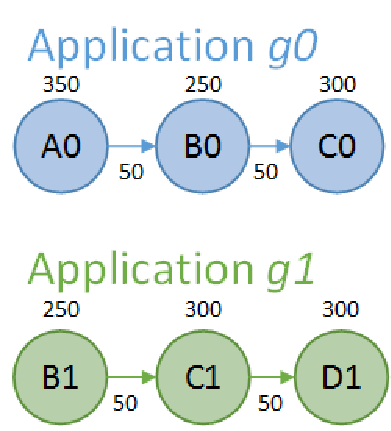
\includegraphics[width=0.9\linewidth]{fig/Apps.pdf}
    \captionof{figure}{Example: Domain Applications}
    \label{fig:Apps}
  \end{minipage}
	 \hfill
  \begin{varwidth}[b]{0.6\linewidth}
    \centering
    \begin{tabular}{l r r r}
      \toprule
      Composition & $P$ & $D_{P}$ & $D_{C}$ \\
      \midrule
      $\{t_A\}$ & 50\% & 350 & -- \\
      $\{t_B\}$ & 100\% & 500 & -- \\
      $\{t_C\}$ & 100\% & 600 & -- \\
      $\{t_D\}$ & 50\% & 300 & -- \\
			\hline
			$\{t_A,t_B\}$ & 50\% & -- & 50 \\
			$\{t_B,t_C\}$ & 100\% & -- & 100 \\
			$\{t_C,t_D\}$ & 50\% & -- & 50 \\
			\hline
			$\{t_A,t_B,t_C\}$ & 50\% & -- & -- \\
			$\{t_B,t_C,t_D\}$ & 50\% & -- & -- \\			
      \bottomrule
    \end{tabular}
    \caption{Example: Domain Features}
    \label{tab:egFeature}
  \end{varwidth}
\end{table}
\subsection{Domain Features}
\label{sec:features}
Domain features lay the foundation for automatic exploration. It is essential to capture behavioral similarity to assess processing needs, and structural similarities to assess communication / topology requirements. Aligned with the domain definition, we identify commonly used functions and function patterns. We express common functions as the function types of actors that repeat within and across applications. Function patterns are repeating compositions these function types (i.e. identical subgraphs). Different lengths of compositions are considered. For example, application $g0$ in Fig.~\ref{fig:Apps}, has three, two and one composition of a degree one, two and three, respectively. The function type composition $\{t_{B}, t_{C}\}$ (which is of degree 2) appears in application $g0$ (actors $B0$,$C0$) and $g1$ ($B1$,$C1$). \tabref{tab:egFeature} lists the compositions of the domain.

%removed the detour of instances. Directly explained it as types. no addl. formula neede
%The definitions of actor composition $c$ and function type composition $C$ are given in Eq.~\ref{eq:comps}.   
%
%\vspace{-10pt}
%%\begingroup\makeatletter\def\f@size{9}\check@mathfonts
%\begin{equation}
%\begin{split}
%\label{eq:comps}
	%c = \{a_j, a_k,...\}, \quad C = \{t_J, t_K,...\}\\
%\end{split}
%\end{equation}
%%\endgroup
%%\vspace{-10pt}

A composition of degree one ($\left\vert{C}\right\vert = 1$) contains a single function type. All compositions $\left\vert{C}\right\vert = 1$, represent the function types shared across the domain. Since compositions $C$ can capture both common functions (behavioral similarity) and function patterns (structural similarity), this paper chooses function type compositions $C$ to express domain features. In addition to the subgraph of function types, we focus on three aspects to characterize compositions: probability of appearance, processing demand and communication demand. 

Compositions that appear more often across applications are more important for the domain than infrequent compositions. To quantify the importance, we define appearance probability $P$ as per Eq.~\eqref{eq:p}. 

%\vspace{-10pt}
\begin{equation}
\begin{split}
\label{eq:p}
P(C_i) = (\sum_{g_j \in G} \left\vert \{ Instance(C_i) \in g_j \} \right\vert) / \left\vert{G}\right\vert \\
%	P(C) = \left\vert{ \{g \vert c \in g, c \in C \} }\right\vert / \left\vert{G}\right\vert \\
\end{split}
\end{equation}


$P$ is probability that an instance of composition $C_i$ appears in a domain application. The composition $\{t_{B}, t_{C}\}$ in Fig.~\ref{fig:Apps} and Table~\ref{tab:egFeature} appears in all applications ($P$ = 100\%). Whereas $\{t_A, t_B\}$ and $\{t_C, t_D\}$ each appear only in one ($P$ =50\%).  

A key challenge to enable domain DSE is how to identify processing and communication demands across applications which are necessary to guide resource allocation. However, considering each individual application is impractical. To obtain a domain-level view, we aggregate the demands for each composition as defined in Eq.~\eqref{eq:demand}.

%\vspace{-8pt}
\begin{equation}
\begin{split}
\label{eq:demand}
	&D_P(C_i=\{t_j\}) = \sum_{g_k \in G} \sum_{ a_l = Instance(t_j) \in g_k} a_l.d_P\\
	&D_C(C_i=\{t_i, t_j\}) = \sum_{g_k \in G} \sum_{e_l \in g_k, e_l=\{t_i,t_j\}} e_l.d_C
\end{split}
\end{equation}
%\vspace{-10pt}

%In general, DSE compares the processing workload $d_P$ among computing actors to decide which to accelerate and analyzes the communication $d_C$ between them to avoid data transfer. However, the individual $d_P$ and $d_C$ is a mess for DS-DSE. The DS-DSE needs the features in domain level to decide the partitioning of function types. 

The processing demand $D_P$ is calculated for each composition $C_i$ with a degree of one as the sum over all applications and all instances of the type $t_j$ (e.g. $D_P(t_B)$ = 500). Communication demand is computed for each pair of actor types (i.e. compositions of degree two). It is the sum of the communication demand for each edge of that type over all applications ($D_C(\{t_B, t_C\})$ = 100). 

%\vspace{-10pt}
\begin{equation}
\begin{split}
\label{eq:CS}
	&CS = \{C_{0}, C_{1}, ..., C_{z}\}\\
	&C_{i} (P, D_P, D_C)\\
\end{split}
\end{equation}
%\vspace{-10pt} 

In summary, the domin features are captured as a set of compositions, where each composition $C_i$ is defined by its appearance probability $P$, processing demand $D_{P}$ (for $\left\vert{C_i}\right\vert = 1$), and communication demand $D_{C}$ (for $\left\vert{C_i}\right\vert = 2$).
Table~\ref{tab:feature} shows the general view of the selected domain features. 

%GSTODO table is redundant in my view
\begin{table}[h]
	\caption{Domain Features}
	\label{tab:feature}
	\centering
	\begin{tabular}{p{0.06\linewidth}|p{0.22\linewidth}|p{0.15\linewidth}|p{0.15\linewidth}|p{0.18\linewidth}}
		\toprule
		\multicolumn{2}{c|}{Composition}& Appearance Probability& Processing Demand& Communication Demand\\
		\midrule
		\hline
		$C_{0}$&				$\{t_{A}\}$&								$P(C_{0})$&					$D_{P}(C_{0})$& --\\
		$C_{1}$& 				$\{t_{B}\}$&								$P(C_{1})$&					$D_{P}(C_{1})$& --\\
		$...$& 					$...$&									$...$&							$...$&	--\\
		$C_{x}$& 				$\{t_{N}\}$&								$P(C_{x})$&					$D_{P}(C_{x})$& --\\
		\hline
		$C_{x+1}$& 			$\{t_{A}, t_{B}\}$&					$P(C_{x+1})$&				--& $D_{C}(C_{x+1})$\\
		$C_{x+2}$& 			$\{t_{A}, t_{C}\}$&					$P(C_{x+2})$&				--& $D_{C}(C_{x+2})$\\
		$...$& 					$...$&									$...$&							--&			$...$\\
		$C_{y}$& 				$\{t_{I}, t_{N}\}$&					$P(C_{y})$&					--& $D_{C}(C_{y})$\\
		\hline
		$C_{y+1}$& 			$\{t_{A}, t_{B}, t_{C}\}$&		$P(C_{y+1})$&				--&	--\\
		$...$& 					$...$&									$...$&							--&	--\\
		$C_{z}$& 				$\{t_{I}, t_{J}, ...,t_{N}\}$&		$P(C_{z})$&					--&	--\\
		\bottomrule
	\end{tabular}
\end{table}
\subsection{Domain Analyzer}
\label{sec:analyzer} 

\newtext{To obtain domain features, domain analyzer extracts the behavioral and structural similarities from the applications within a domain. It expresses these similarities using the domain features defined in} \secref{sec:features}. The computed domain features then feed into our domain-specific DSE described in \secref{sec:DSE}.
%This paper primarily focuses on streaming applications, which have significant functional and structural similarities within a domain. The extracted similarities 

Algorithm~\ref{alg:analysis} overviews the domain analyzer. The analyzer is comprised of domain analysis and application analysis. The domain analysis (lines 1-11) first calls application analysis for each application to obtain the list of function type compositions ($CList$ in line3). Then the domain analysis merges compositions from all applications, counts their appearance frequency (lines 4-8), and aggregates their processing and communication demand ($D_P, D_C$ in line 9). Finally, the domain analysis calculates each composition appearance probability ($P$ in line 11) and returns the the domain features as a set of function type compositions.

\begin{algorithm}
\caption{Domain Analyzer}
\label{alg:analysis}
\begin{algorithmic}[1]
{\footnotesize
\Function{dmAnalysis}{$G$}
	\For{\textbf{each} $g \in G$}
		\State $CList = \Call{appAnalysis}{g}$
		\For{\textbf{each} $C \in CList$}
				\If {$C \in CS$}
					\State $Freq(C)$++
				\Else
					\State $CS = CS \cup \{C\}; Freq(C) = 1$
				\EndIf
				\State $D_{P}(C)$ += $C.D_{P}; D_{C}(C)$ += $C.D_{C}$
		\EndFor
	\EndFor
	\For{\textbf{each} $C \in CS$}
		\State $P(C) = Freq(C) / \left\vert{G}\right\vert$
	\EndFor
	\Return $CS$
\EndFunction
\item[]
\Function{appAnalysis}{$g$}
	\For{\textbf{each} $a \in g.A$}
		\State $cList.add( \{a\} )$
	\EndFor
	\For{$k \in \{1,2,\dots\}$}
	\Comment $k$ is composition degree
		\For{\textbf{each} $c \in\{cList \cap \left\vert{c}\right\vert = k\}$ }
			\For{\textbf{each} $a_{next} \gets c.a_{tail}().a_{outNeighbor}()$}
				\If{$a_{next} \notin c$}
					\State $cList.add( c \cup \{a_{next}\} )$
				\EndIf
			\EndFor
		\EndFor
		\IIf {$\{c \vert c \in cList \cap \left\vert{c}\right\vert = k$+$1\} = \emptyset$} Break
	\EndFor

	\For{\textbf{each} $c \in cList$}
			\State $C$ = \{$a.t \vert a \in c$\}
			\IIf {$\left\vert{c}\right\vert = 1$} $C.D_{P} = a.d_{P},$ which $a \in c$
			\IIf {$\left\vert{c}\right\vert = 2$} $C.D_{C} = e.d_{C},$ which $ e.a_{src,dst} \in c$
			\If {$C \in CList$}
				\State $CList[C].updateD(C.D_{P},C.D_{C})$
			\Else
				\State $CList.add(C)$
			\EndIf
	\EndFor
	\Return $CList$
\EndFunction
}
\end{algorithmic}
\end{algorithm}

The application analysis (lines 12-28) creates a list of actor compositions (lines 12-20) and then abstracts from actor instances into function type compositions (lines 21-28). The analysis starts with each actor from the application as 1-degree composition (lines 13-14). Then for each $k$-degree composition, it adds one more actor to it to build a $k+1$ degree composition (lines 15-19). When no actor can be added anymore, actor compositions detection stops (line 20). After that, the analysis obtains a function type composition from each actor composition(lines 21-22). It merges duplicated function type compositions and aggregates their processing/communication demand (lines 23-28). It returns the list of compositions of this application, with their aggregated processing and communication demands. 
%The extracted similarities will be used as the input model for our proposed domain-specific DSE.






% GA domain formalization

%A domain is a set of applications, which share common functions and common patterns as introduced in \cite{zhang100ds}. Eq.~\ref{eq:domain} presents domain concept symbolically. A domain $G$ is a set of streaming applications ($g_{0}$ .. $g_{N}$), each captured as a dataflow graph \cite{stuijk2006sdf}. Each application $g_i$ contains a set $A$ of processing actors ($a_0$ .. $a_n$) and a set of $E$ edges ($e_0$ .. $e_m$) representing the communication between actors. Each actor $a_i$ is an instance of a function type $t$ with an instance-specific processing demand $d_{P}$ (\# of operations\footnote{To simplify explanation and clarity in result discussion, we abstract processing to a single dimension. More dimensions are possible and only affect the evaluation.}). Multiple instances of the same function type $t$ may exist within and across applications within the domain. A domain contains a set $T$ of function types. Each edge $e_i$ is the directed communication $a_{src}$ to $a_{dst}$ with a communication demand of $d_{C}$ (\# of transferred bytes). 

%\begin{equation}
%\begin{split}
%\label{eq:domain}
%	&G = \{g_{0}, g_{1}, ..., g_{N}\}, \quad g_{i} = (A, E)\\
%	&A = \{a_{0}, a_{1}, ..., a_{n}\}, \quad E = \{e_{0}, e_{1}, ..., e_{m}\}\\
%	&a_{i} (t, d_{P}), \quad e_{i} ((a_{src}, a_{dst}), d_{C})\\
%		&T = \{t_{A}, t_{B}, ..., t_{X}\}
%\end{split}
%\end{equation}

% potentially move this defintion to GALS approach.
%Given the formalization, the problem can be defined as follows:
%\begin{problem}[DS-DSE]
%\label{p:dse}
%	\normalfont{Given a domain \textit{G} and a HW budget $N$ (area), find a HW/SW partition of \textit{T} (the set of domain function types) that maximizes average throughput improvement over pure SW execution for all $\textit{g} \in \textit{G}$.}
%\end{problem}